%*********************************************************************
%	CHAPTER 6 - 3D RECONSTRUCTION
%*********************************************************************
\chapter{3D Reconstruction}
\label{ch:reconstruction}
%=====================================================================
% SECTION: Introduction
%=====================================================================
\section{Introduction}
\label{sec:ch5.reconstruction_intro}
This chapter evaluates the accuracy and coverage of the stereo reconstruction pipeline in underwater conditions.
Two datasets (\hyperref[sec:ch4.ds2]{DS2}, \hyperref[sec:ch4.ds3]{DS3}) are used to evaluate the accuracy and coverage of the 
pipeline.

The pipeline is built and tested one stage at a time. The reconstruction is broken into three
stages:

\begin{enumerate}
    \item \textbf{\hyperref[sec:ch5.stereo_depth]{Depth per frame}:} Stereo pairs are used to generate depth maps.
    \item \textbf{\hyperref[sec:ch5.pose_estimation]{Pose per frame}:} The camera's position and orientation within the world frame.
    \item  \textbf{\hyperref[sec:ch5.frame_integration]{Fusion}:} Combining the separate point clouds into a single object.
\end{enumerate}

Each stage is then covered in its own section, which follows the same structure. The methods evaluated are first described,
 together with the theory underlying their specific
implementations. The experimental procedure is then outlined, after which the results are presented and analysed.


Stereo matching is evaluated first (\autoref{sec:ch5.stereo_depth}), comparing OpenCV's implementation of
Semi-Global Matching (SGBM) \cite{hirschmullerStereoProcessingSemiglobal2008} with two learnt models,
FoundationStereo \cite{wenFoundationStereoZeroShotStereo2025} and AquaStereo
\cite{weiAquaStereoEnablingUnderwater2026}. Pose estimation using AprilTags, ICP and COLMAP is then compared
(\autoref{sec:ch5.pose_estimation}), followed by frame fusion using COLMAP and a TSDF
(\autoref{sec:ch5.frame_integration}). The choices made at each stage carry forward into the next. The complete
pipeline is then tested as a whole, including its dependence on the number of frames
(\autoref{sec:ch5.testing_full_pipeline}). Finally, the results are summarised in \autoref{sec:ch5.summary}.


%=====================================================================
% SECTION: Depth Estimation
%=====================================================================
\section{Depth Estimation}
\label{sec:ch5.stereo_depth}
% The disparity equation, the correspondence problem, and then SGBM, FoundationStereo and AquaStereo
% Maths done in intro depth per pixel
% Rough explain OpenCVSGBM, FoundationStereo, AquaStereo, COLMAP (different approach)
% Show breif comparison with analysis - NOt sure what metric

As derived in \autoref{subsec:ch3.disparity}, the depth $Z$ of any point is found from its disparity using: 
\begin{equation}
    Z = \frac{fB}{d},
\end{equation}
where $f$ is the focal length in pixels and $B$ is the baseline between the two cameras.
The equation is simple but the difficulty lies in determining $d$, which requires matching each pixel in the left image to the same point
in the right image. Areas with little texture look near identical between pixels, meaning many matches are possible. 
Patterns that repeat throughout the image produce several candidate matches that may all look correct. Parts of the scene may be visible from only one camera
but occluded from the other, resulting in no match at all. Underwater, these problems are made worse because scattering and attenuation 
reduce image contrast \cite{roserSimultaneousUnderwaterVisibility2014}.
Three depth estimation methods are compared in this section, each approaching the correspondence problem differently. 

\subsection{Stereo Matchers}
\label{subsec:ch5.stereo_matchers}
% ~~~~~ Subsubsection: OpenCV SGBM ~~~~~
% TODO: De-claudify
\subsubsection{OpenCV SGBM}
% COmpares small blocks of pixels
Semi-Global Block Matching (SGBM) is a classical approach, used within this
project through OpenCV~\cite{opencv_sgbm}. For each pixel $\mathbf{p}$ and
candidate disparity $d$, it computes a matching cost $C(\mathbf{p}, d)$. This is done by
comparing a small block around $\mathbf{p}$ in the left image with the block
shifted by $d$ in the right image, using the Birchfield--Tomasi
measure~\cite{birchfield1998}. Following
Hirschmüller~\cite[Eq.~(11)]{hirschmullerStereoProcessingSemiglobal2008}, it
then seeks the disparity map $D$ that minimises
\begin{equation}
    E(D) = \sum_{\mathbf{p}} \Big( C(\mathbf{p}, D_\mathbf{p})
    + \sum_{\mathbf{q} \in N_\mathbf{p}} P_1 \, T\big[|D_\mathbf{p} - D_\mathbf{q}| = 1\big]
    + \sum_{\mathbf{q} \in N_\mathbf{p}} P_2 \, T\big[|D_\mathbf{p} - D_\mathbf{q}| > 1\big] \Big),
    \label{eq:sgm_energy}
\end{equation}
where $N_\mathbf{p}$ are the neighbours of $\mathbf{p}$ and $T[\cdot]$ is 1
when its condition is true and 0 otherwise. The penalty $P_1$ allows
slow depth changes, while the larger $P_2$ minimises sudden jumps unless
the matching cost strongly supports them, such as at object edges. SGBM
approximates this minimisation by combining costs along multiple straight
paths through the image, with each pixel taking the disparity with the lowest
combined cost. SGBM is fast but relies on local pixel similarity, so it
struggles in regions of weak texture~\cite{kendallEndtoEndLearningGeometry2017}.


% Maybe include the equation for how it works
% ~~~~~ Subsubsection: Learnt Models ~~~~~
\subsubsection{Learnt Models}
Learnt models train on features from large datasets, replacing the designed matching costs with learnt features. Classical methods compare raw pixels, so they struggle in textureless
and repetitive environments. Learnt models instead compare learnt feature descriptors of each image region,
allowing them to use wider semantic context \cite{kendallEndtoEndLearningGeometry2017}.
The weakness however is that they depend heavily on training data \cite{wenFoundationStereoZeroShotStereo2025}.
For this reason, two different learnt models are tested, a leading general-purpose model trained on a very large dataset, and a model designed specifically for underwater use. 
\autoref{fig:gcnet-architecture} shows the forward pass of GC-Net \cite{kendallEndtoEndLearningGeometry2017}, 
an early end-to-end learnt stereo model whose cost volume and soft argmin regression later models build on.


% GC-Net's forward pass
\begin{figure}[htbp]
  \centering
  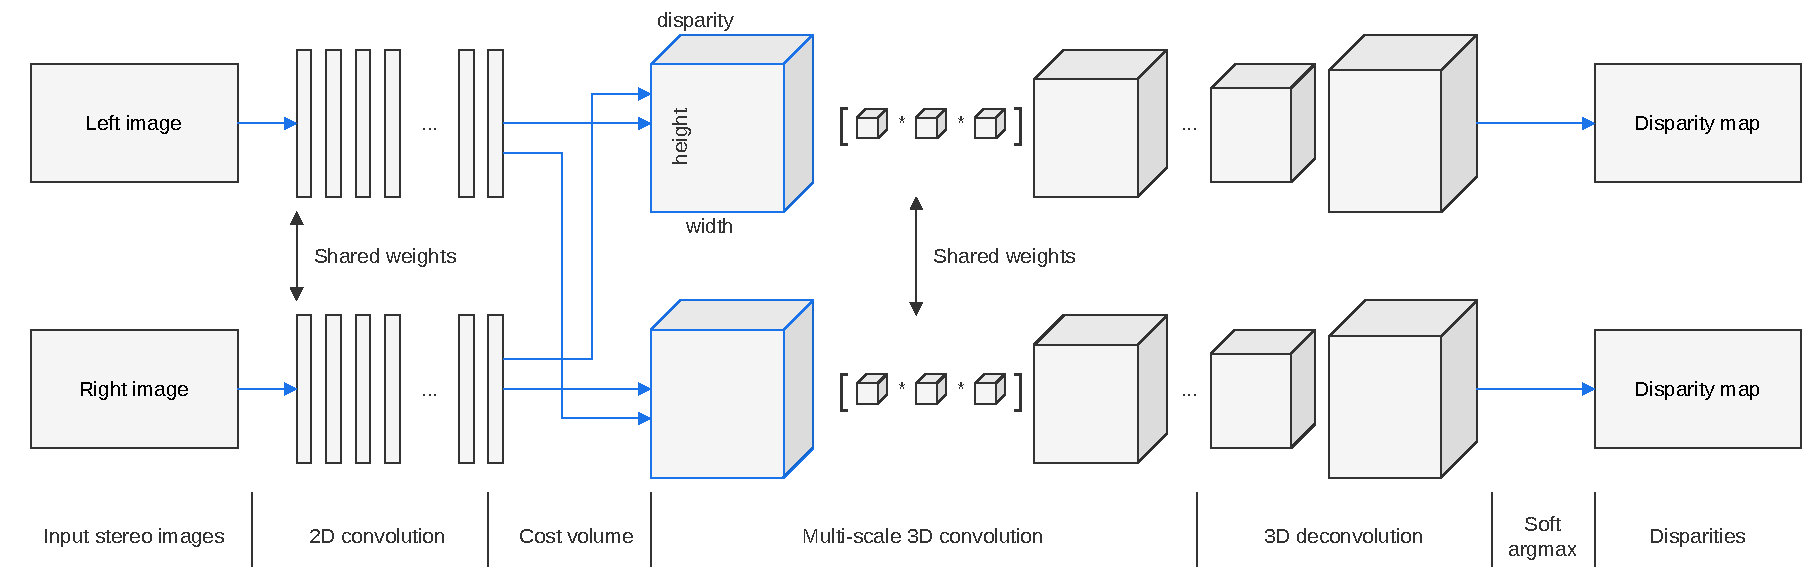
\includegraphics[width=\textwidth]{figs/Ch5/gcnet-architecture.drawio.pdf}
  \caption[GC-Net forward pass]{Forward pass of GC-Net. A rectified stereo pair passes through shared-weight 2D convolutions; the resulting features form a 4D cost volume, which 3D convolutions and deconvolutions regularise before a soft argmin regresses the disparity map. Adapted from Kendall et al.~\cite{kendallEndtoEndLearningGeometry2017}.}
  \label{fig:gcnet-architecture}
\end{figure}
% MAKE own diagram to explain how they work.

\textbf{FoundationStereo} \\
FoundationStereo is an NVIDIA general-purpose model trained on roughly one million synthetic stereo pairs. 
It is designed to generalise to new scenes without any fine-tuning, making it zero-shot. It utilises a pretrained monocular depth model and compares every possible disparity
to build a cost volume. This volume is filtered with 3D convolutions and a mechanism that weighs each pixel's candidate disparity against the others.
The resulting disparity map is refined iteratively. Further details on the model architecture, training and benchmark results are given
in the \href{https://doi.org/10.1109/CVPR52734.2025.00495}{\textcolor{blue}{original paper}} \cite{wenFoundationStereoZeroShotStereo2025} and the
\href{https://github.com/NVlabs/FoundationStereo}{\textcolor{blue}{official implementation}}.

\textbf{AquaStereo} \\
AquaStereo is a learnt model designed specifically for underwater reconstruction. Because little underwater training data exists, it uses synthetic underwater stereo pairs, 
generated from an in-air dataset. During training, a teacher model predicts disparity from the clean in-air images, and AquaStereo learns to reproduce the
same predictions from low-texture, turbid versions of the same images \cite{weiAquaStereoEnablingUnderwater2026}.



\subsection{Test Setup}
\label{sec:ch5.depth_test}
% Write a test script to do the following. It needs to be able to take in of images and apply technique (these are input params)
% Also have input param for output folder
% Run on S30 and sun/py2_frames_pass1 and shade/pyr1_frames_pass4_730mm
% 1. Depth map generation
% - Use the three matchers (SGBM, AquaStereo, FoundationStereo) to generate depth maps. Generate images for each frame.
% - Metrics are total points per frame (median)
% For each approach, generate an image that indicates for a report how it maps between the two images (e.g. lines between keypoints)
% This code needs to be written such that I can easily repeat the tests


% What is tested
This test measures how effectively each stereo matcher produces depth maps. Seven recordings were used: a side-on scan of the
3D-printed targets at 30\,cm (S30, 69 frames, \hyperref[sec:ch4.ds2]{DS2}), and six upward-facing scans of the ice targets (\hyperref[sec:ch4.ds3]{DS3}), with
the pyramid, cubes, overhang and wave in shade, and the pyramid and overhang in strong sunlight.
The matchers are compared on coverage, the share of the image with depth inside the recording's depth range, and
on the number of points, counted as occupied 1\,mm voxels in the point cloud.
Accuracy is only examined in the 3D reconstruction tests in \autoref{subsec:ch5.fusion_results}.

The four configurations were tested as summarised in \autoref{tab:matcher_settings} below. 
Each method is tested in the pipeline's depth code, \texttt{depth\_frames.py}. 
SGBM was run with both its default settings and a tuned configuration. 
% TODO: ADD SCANS OF ALL OTHER SHAPES TO APPENDIX

\begin{table}[htbp]
    \centering
    \caption{Stereo matcher configurations used in the depth map test.}
    \label{tab:matcher_settings}
    \begin{tabularx}{\textwidth}{@{}lX@{}}
        \toprule
        \textbf{Method} & \textbf{Settings} \\
        \midrule
        SGBM, default    & 8-path mode (\texttt{MODE\_HH}), block size 9, uniqueness 5,
                           speckle filter, left-right check 1\,px \\
        SGBM, tuned      & Half scale, block size 11, uniqueness 0,
                           $P_1/P_2 = 16/32$, pre-filter cap 63 \\
        AquaStereo       & ViT-B backbone, half scale, 32 refinement iterations,
                           left-right check 3\,px \\
        FoundationStereo & ViT-L backbone, half scale, 32 refinement iterations,
                           left-right check 3\,px, 416\,px disparity range \\
        \bottomrule
    \end{tabularx}
\end{table}




% SGBM Basics, SGBM after parameter sweep

% Output image comparing

\subsection{Results}
\label{subsec:ch5.depth_results}

\autoref{tab:depth_matchers_summary} summarises the coverage of each matcher, averaging the recordings and
separating them by lighting conditions. The full table is given in the appendix (\autoref{tab:depth_matchers}). \autoref{fig:ch5.depth_crops}
shows the depth maps generated for each ice shape, and \autoref{fig:ch5.depth_crops_sun} compares the depth maps of
the stepped pyramid ice in sunny and shaded conditions.

\begin{table}[H]
    \centering
    \caption{Depth map generation per matcher on the ice: averaged (mean) over the DS3 ice recordings in \autoref{tab:depth_matchers}.
    Coverage in \%,
    points in thousands.}
    \label{tab:depth_matchers_summary}
    \begin{tabular}{lrrrr}
        \toprule
                         & \multicolumn{2}{c}{Shade (4 recordings)} & \multicolumn{2}{c}{Sun (2 recordings)} \\
        \cmidrule(lr){2-3}\cmidrule(lr){4-5}
        Matcher          & Coverage & Points & Coverage & Points \\
        \midrule
        SGBM             & 15.3     & 185    & 9.8      & 110    \\
        SGBM (tuned)     & 22.6     & 259    & 17.1     & 176    \\
        AquaStereo       & 16.7     & 171    & 11.9     & 82     \\
        FoundationStereo & 30.1     & 372    & 15.8     & 102    \\
        \bottomrule
    \end{tabular}
\end{table}


\subsubsection{Coverage in Shade}

On the four shaded ice recordings, FoundationStereo produced the most depth, with a mean coverage of 30.1\,\% compared
to 22.6\,\% for the tuned SGBM. The gap is largest for the wave block, where FoundationStereo covered 41.2\,\% of the
image against a second best of 19.0\,\% for the tuned SGBM. Based on the coverage metric, AquaStereo appears to be
outperformed by the tuned SGBM; however, \autoref{fig:ch5.depth_crops} tells a different story. Both learnt models
concentrate their coverage on the scanned ice shapes, whereas the SGBM implementations have speckled noise all
around the image, which adds to their coverage.

\begin{figure}[H]
    \centering
    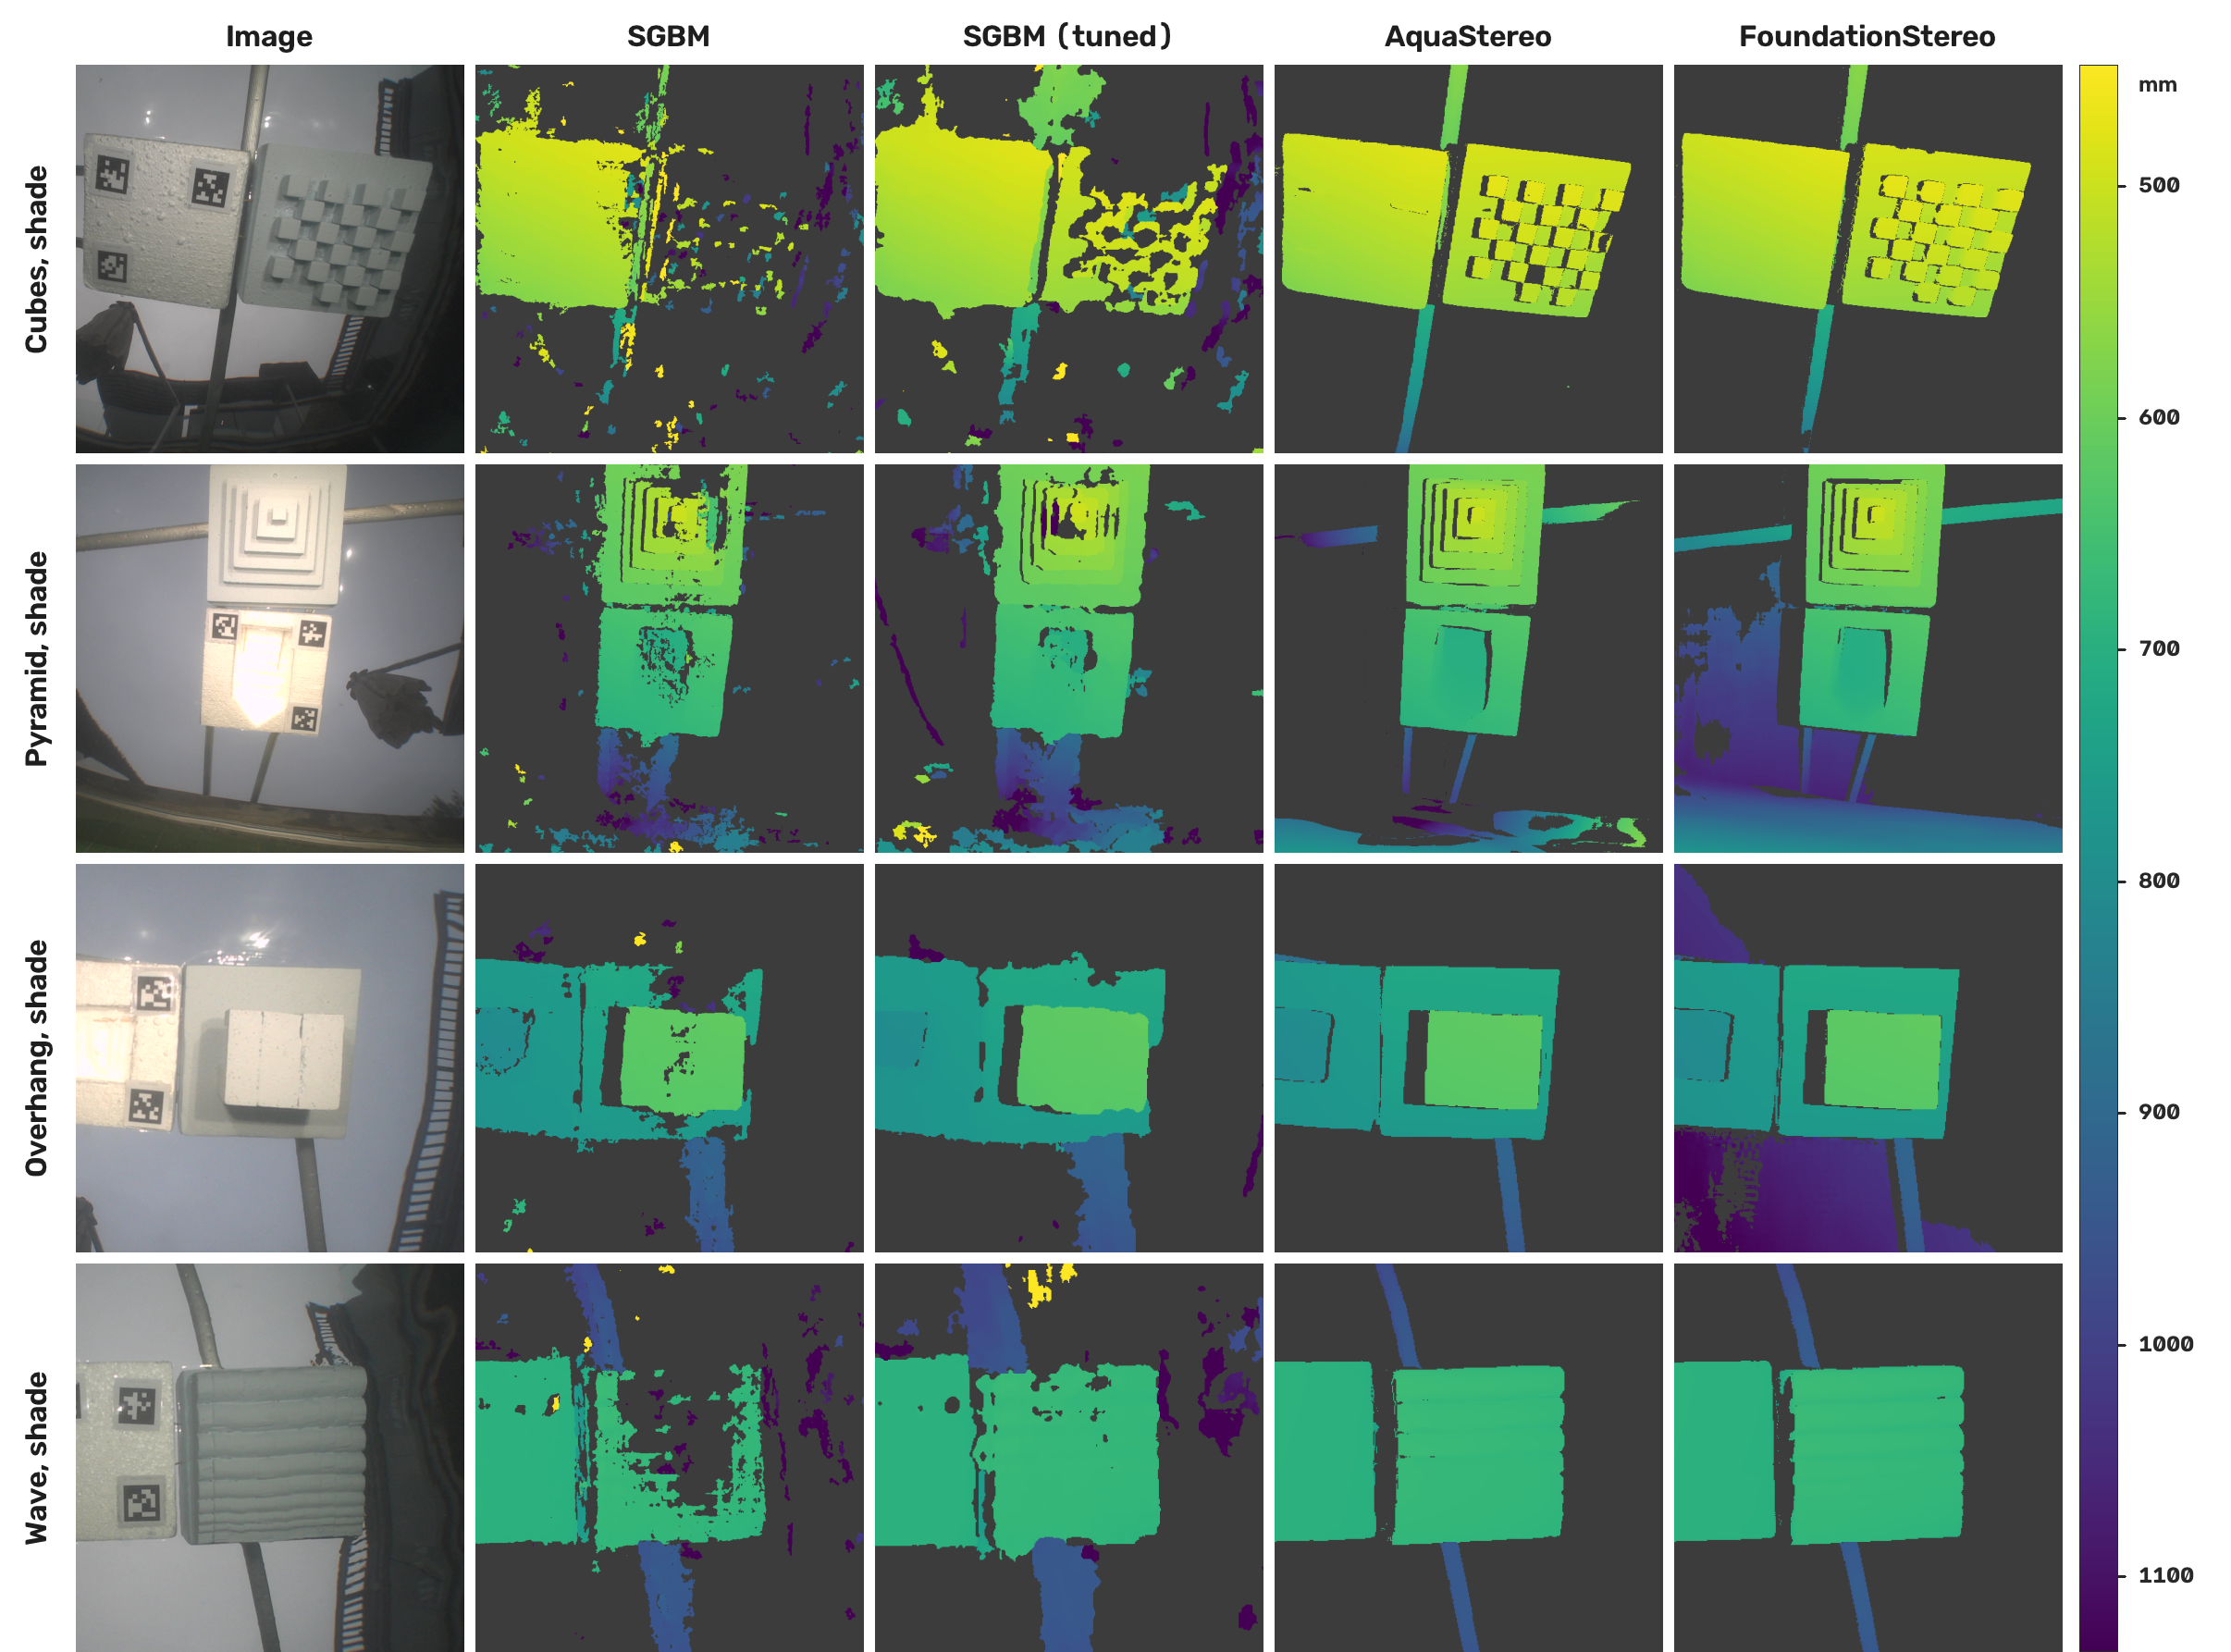
\includegraphics[width=\textwidth]{figs/Ch5/depth_comparison_4.png}
    \caption[Depth maps of the shaded ice scans]{\textbf{Depth maps of the shaded ice scans.} Rectified left image
    and each matcher's depth map for one frame of each recording, on one depth scale (447--1132\,mm); grey has no
    depth.}
    \label{fig:ch5.depth_crops}
\end{figure}


\subsubsection{Impact of Direct Sunlight}

The backlighting in full sun reduced the coverage of all matchers as shown in \autoref{fig:ch5.depth_crops_sun}. FoundationStereo fell from
30.1\,\% to 15.8\,\% and AquaStereo from 16.7\,\% to 11.9\,\%, while the tuned SGBM fell least, from 22.6\,\% to 17.1\,\%, and
produced the most points in sunny conditions. As in the shaded conditions, however, the coverage metric is
misleading. Most of the SGBM depth is scattered speckle with no true surface present. FoundationStereo produced
fewer depth points, but almost all of them lie on the pyramid. FoundationStereo recovers the full stepped shape of
the pyramid and AquaStereo its outer steps, while the SGBM implementations become overrun with noise.

\begin{figure}[H]
    \centering
    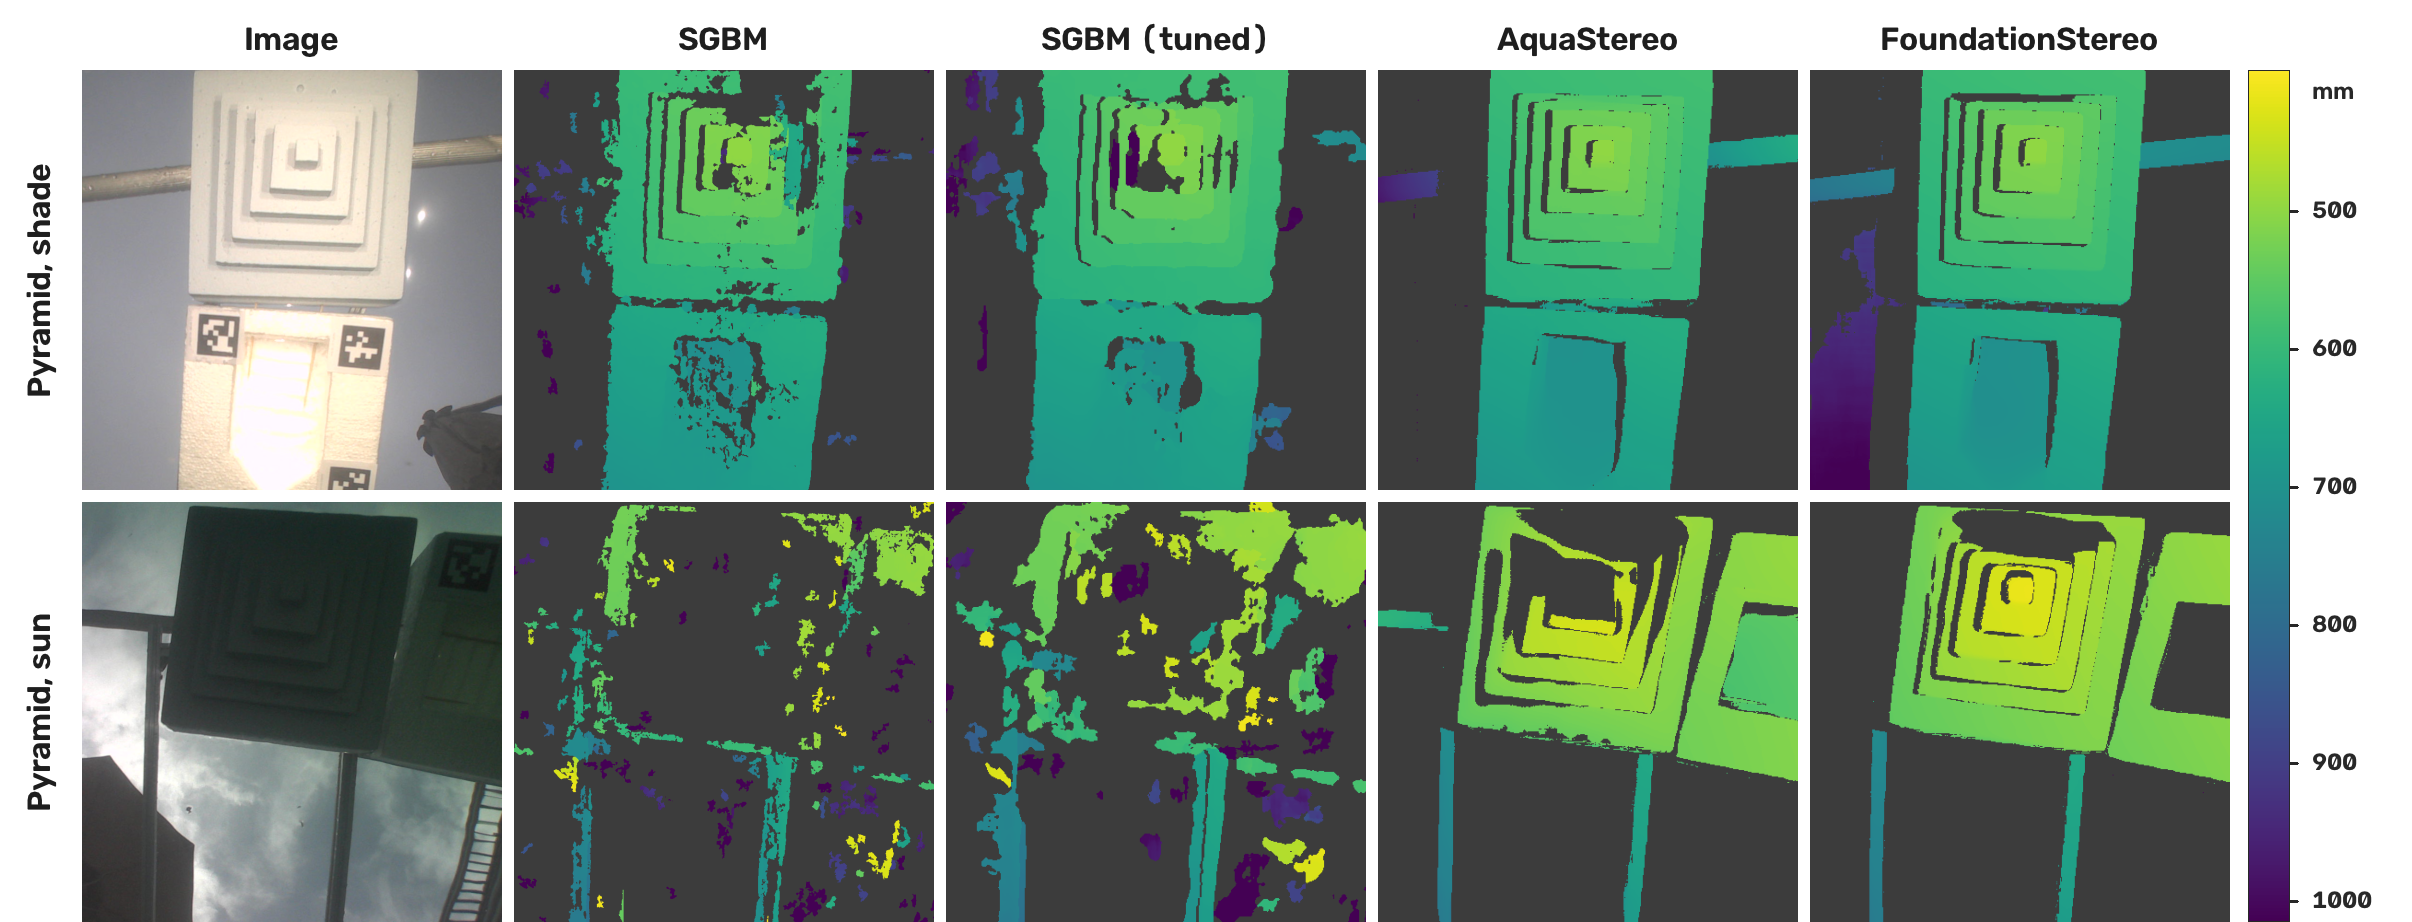
\includegraphics[width=\textwidth]{figs/Ch5/depth_comparison_sun_shade.png}
    \caption[Pyramid ice depth in shade and sun]{\textbf{Effect of backlighting on depth.} Pyramid ice in shade
    (top) and backlit by the sun (bottom): rectified left image and each matcher's depth map, on one depth scale
    (394--1068\,mm). Grey has no depth.}
    \label{fig:ch5.depth_crops_sun}
\end{figure}


\subsection{Discussion}
\label{subsec:ch5.depth_discussion}

Across the ice scans, FoundationStereo gave the most complete depth on the targets in shade and was the only
matcher to keep the full ice shape when backlit. It was therefore selected as the primary depth generator for the
remaining pipeline steps, with tuned SGBM kept for comparison as the best classical matcher.


 
%=====================================================================
% SECTION: Pose Estimation
%=====================================================================
\section{Pose Estimation}
\label{sec:ch5.pose_estimation}
% This section is background theory about the exact approaches chosen. In Th
\autoref{sec:ch5.stereo_depth} examines how depth can be generated from an image. 3D reconstruction, however, requires multiple
viewpoints of the same scene. To merge these frames together, the camera's position relative to the scene must be known, which requires pose
estimation. This can be done in a number of ways, three of which are explained and tested in this section.

\subsection{Pose Methods}
\label{subsec:ch5.pose_methods}
%---------------------------------------------------------------------
% Subsection: Using Tag poses
%---------------------------------------------------------------------
\subsubsection{AprilTag Poses}
\label{subsec:ch5.tag_poses}
AprilTags are useful beyond creating an occlusion-friendly calibration board. Placing AprilTags within a scene
creates easily identifiable locations. The camera's position can be calculated from the 3D positions of these corner locations and 
is implemented in \texttt{tag\_poses.py}. The pose is found by computing the rotation and translation that best
align the tag map with the measured corners \cite{umeyamaLeastsquaresEstimationTransformation1991}, and inverting it.
 
\begin{figure}[H]
    \centering
    \includegraphics[width=1 \textwidth]{../Diagrams/TagPosePipeline.pdf}
    \caption{AprilTag pose estimation: tag corners are triangulated, mapped across all frames, and aligned to each frame to recover the camera pose.}

    \label{fig:ch5.TagPosePipeline}
\end{figure}
Each frame's pose is independent, meaning errors do not accumulate over time. This method does, however, require the tags to be visible within the frames and
inherits any calibration and distortion error.


%---------------------------------------------------------------------
% Subsection: ICP (Iterative Closest Point)
%---------------------------------------------------------------------
\subsubsection{ICP (Iterative Closest Point)}
\label{subsec:ch5.icp}
% EXPLAIN
ICP (Iterative Closest Point) is a standard technique for aligning 3D point clouds \cite{besl1992}.
Here it is used to estimate camera motion from the shape of each frame's 3D point cloud. Each new frame's point 
cloud is shifted and rotated until it matches a reference cloud.
The amount of movement between clouds is the amount the camera has moved. 

First, each frame's stereo depth map is converted into a 3D point cloud with
one point per valid pixel. Each cloud is reduced to one point per 4\,mm cube
(voxel), and each point is given a surface normal, estimating the direction
of its surface. The algorithm then works off a starting guess, assuming each
new frame repeats its last motion. It then pairs each point with its nearest
neighbour in either the last frame or the last 10 frames. It shifts and
rotates the cloud until it fits as closely as possible, repeating the pairing each
 time \cite{besl1992}. Each frame's motion is combined with the previous pose to generate
\texttt{T\_cam\_world}.
% VISUALISE
\begin{figure}[H]
    \centering
    \includegraphics[width=1 \textwidth]{../Diagrams/ICPPipeline.pdf}
    \caption{ICP pose estimation: each frame's point cloud is aligned to a reference cloud and the motions are chained into a trajectory.}
    \label{fig:ch5.ICPPipeline}
\end{figure}


% ADD IMAGE SHOWING IT WORKING - WHERE THE DETECTIONS ARE?

% IMPLICATIONS
ICP needs no markers, but is heavily dependent on the depth method chosen. Noisy or incomplete depth maps lead to poor alignment. Because each pose is built on the one before,
errors accumulate and the estimated trajectory drifts over time.


%---------------------------------------------------------------------
% Subsection: COLMAP
%---------------------------------------------------------------------
\subsubsection{COLMAP}
\label{subsec:ch5.colmap}
Unlike ICP, COLMAP uses texture rather than shape. It finds distinctive patterns in each image and matches them across frames, then uses the matches to recover both
the camera poses and the 3D positions of the matched points, a process called Structure from Motion (SfM) \cite{schonberger2016sfm}.
First, SIFT (Scale-Invariant Feature Transform) is used to find keypoints in both left and right images \cite{lowe2004}.  SIFT describes each keypoint with a vector that
summarises the brightness gradients in the surrounding patch, which stays
largely unchanged under changes in scale, rotation and lighting.  This means the same physical point can be recognised from different viewpoints. 
Keypoints are then matched between frames within $\pm 12$ frames of each other. The reconstruction is built incrementally.
As frames are added, bundle adjustment optimises camera poses and 3D points to minimise the reprojection error, the difference between
where each 3D point projects into an image and where the keypoint was actually detected \cite{triggs2000}. Each frame's pose is read out as \texttt{T\_cam\_world}.

\begin{figure}[H]
    \centering
    \includegraphics[width=1 \textwidth]{../Diagrams/COLMAPPipeline.pdf}
    \caption{COLMAP pose estimation: SIFT keypoints are matched between nearby frames and the poses are refined incrementally by bundle adjustment.}
    \label{fig:ch5.COLMAPPipeline}
\end{figure}

SIFT relies on texture to find keypoints, meaning COLMAP can struggle on plain or blurred surfaces with few distinctive keypoints \cite{lowe2004}. 




\subsection{Test Setup}
% 2 pages max
% Write a script that can compare all 3 pose estimation apptoaches. It needs to fit within the standard
% reconstruction pipeline and be easily repeatable.
% Compare all 3 on the same data used in the Depth tests
% Output images that show the DETECTIONpoints (SIFT + ICP) for my report
% COLMAP, ICP on FoundationStereo, ICP on SGBM, AprilGRid.
% NOt sure the metrics to compare, lets have this discussion before you begin.
% Specifiy what mode each was run in (list)




\label{subsec:ch5.methods_tested}
Four different pose methods are tested. To stop the AprilTags being used as matching points, particularly by SIFT
which relies on texture, the tags are automatically masked out of the images given to every method except
AprilGrid. COLMAP’s feature extraction ignores the masked pixels, and they are left out of the depth maps used by ICP.


\label{subsec:ch5.methods_tested_error}
\begin{enumerate}
    \item \textbf{AprilTags} (\texttt{tag\_poses.py}): the reference, and the only method that sees the tags.
    Tag corners are triangulated in stereo, rejecting tags with a reprojection error above 0.8\,px.
    \item \textbf{COLMAP} (\texttt{colmap\_poses.py}): SfM on SIFT features (GPU), with the intrinsics and stereo
    configuration fixed from the calibration.
    \item \textbf{ICP, FoundationStereo} (\texttt{depth\_frames.py} + \texttt{icp\_poses.py}): each frame's depth map
    is registered by point-to-plane ICP onto a local map of the last 10 frames.
    \item \textbf{ICP, SGBM}: as above, with depth from the tuned SGBM matcher.
\end{enumerate}


% TO BE DONE OVERNIGHT AND TOMORROW MORNING

\label{subsec:ch5.evaluating_pose_estimations}
From each pose method, camera trajectories were generated across the full scan. These trajectories are compared against the AprilTag-generated poses. 
Accuracy is measured using absolute trajectory error (ATE) \cite{sturmBenchmarkEvaluationRGBD2012}. Each trajectory is aligned to the AprilGrid reference and the
distance between the two is measured at every frame.

%===================
\subsection{Results}
\label{subsec:ch5.pose_results}
\subsubsection{Trajectory Accuracy}
% TBH maybe just write about this section, and refrence the appendix
% Failed to detect AprilTags on the sun one. 
% Show table with all the errors 

The upward-facing pyramid scan in full sun has multiple frames only containing a single AprilTag. This results in a poor ground-truth trajectory. For this scan, the comparison
is purely based on the visual trajectory in \autoref{fig:ch5.trajectories}, where the estimated ground-truth pose is also plotted.



\begin{table}[H]
\centering
\caption{Absolute trajectory error (ATE) of each pose method relative to the
AprilGrid reference, after a single rigid alignment. ATE is not reported for
the sunlit recording, where the reference is too noisy for a reliable
comparison.}
\label{tab:pose_comparison}
\small
\setlength{\tabcolsep}{3pt}
\begin{tabular*}{\textwidth}{@{\extracolsep{\fill}}lccccccccc@{}}
\toprule
 & \multicolumn{3}{c}{Pyramid Ice, shade} & \multicolumn{3}{c}{Pyramid Ice, sun} & \multicolumn{3}{c}{S30} \\
\cmidrule(lr){2-4}\cmidrule(lr){5-7}\cmidrule(lr){8-10}
 & Frames & \multicolumn{2}{c}{ATE (mm)} & Frames & \multicolumn{2}{c}{ATE (mm)} & Frames & \multicolumn{2}{c}{ATE (mm)} \\
Method & posed & RMSE & max & posed & RMSE & max & posed & RMSE & max \\
\midrule
AprilGrid             & 151/151 & ref.  & ref.  & 118/151 & ref. & ref. & 280/344 & ref. & ref.  \\
COLMAP                & 151/151 & 6.79  & 22.26 & 151/151 & --   & --   & 344/344 & 2.43 & 6.44  \\
ICP, FoundationStereo & 135/151 & 24.98 & 70.11 & 150/151 & --   & --   & 340/344 & 2.89 & 7.14  \\
ICP, SGBM (tuned)     & 151/151 & 30.31 & 70.92 & 1/151   & --   & --   & 338/344 & 5.91 & 16.08 \\
\bottomrule
\end{tabular*}
\end{table}

All three methods follow the shaded trajectory closely, with ATE values between 6.8 and 30.3\,mm
(\autoref{tab:pose_comparison}). 
COLMAP outperforms both ICP runs in the shade, with roughly four times lower error. 
The sunlit pass, however, gives very different results. ICP with SGBM fails completely, estimating a pose only for its first frame. 
COLMAP registers some images but is far from the reference path, jumping  between frames. 
ICP with FoundationStereo is the only algorithm that tracks the camera throughout the sunlit pass.
% Have it four seperate figures
% Show trajectory mapping for shadow ice.
\begin{figure}[H]
    \centering
    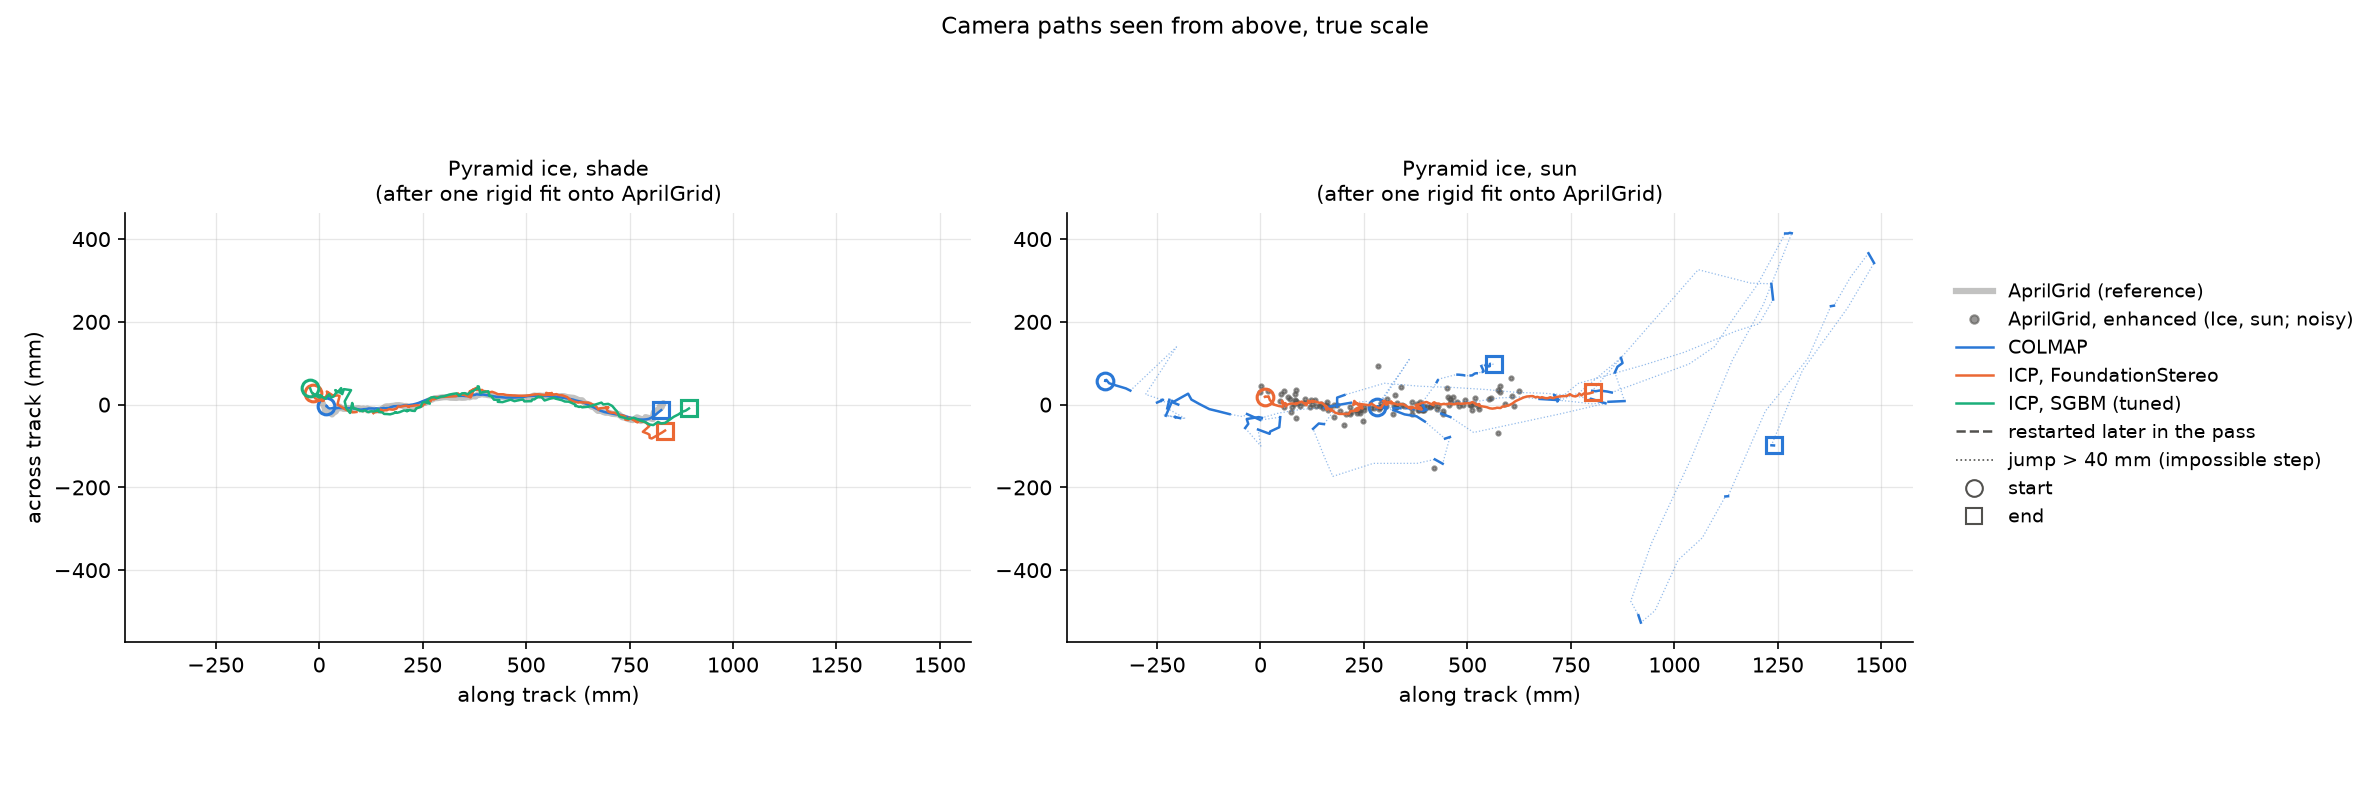
\includegraphics[width=1 \textwidth]{figs/Ch5/paths_ice_shade_sun.png}
    \caption{Camera paths from above at true scale, each rigidly aligned to the AprilTag poses. 
    In sunlight, the reference is a noisy single-tag estimate and ICP with SGBM lost track immediately. 
    Dotted segments are frame-to-frame jumps greater than 40\,mm.}
    \label{fig:ch5.trajectories}
\end{figure}


\subsubsection{Feature Detection}
Each algorithm relies on different features. As shown in \autoref{fig:ch5.shadow_ice_detections}, 
COLMAP's SIFT detects and matches far fewer points than the ICP methods, both across the image and on the ice target itself. 
All three markerless methods also use features outside the ice target for matching, 
including an umbrella above it and the pole securing the target. Visually, the SGBM ICP points appear more scattered,
 whereas the COLMAP and FoundationStereo ICP points cluster around real objects in the frame.



\begin{figure}[H]
    \centering
    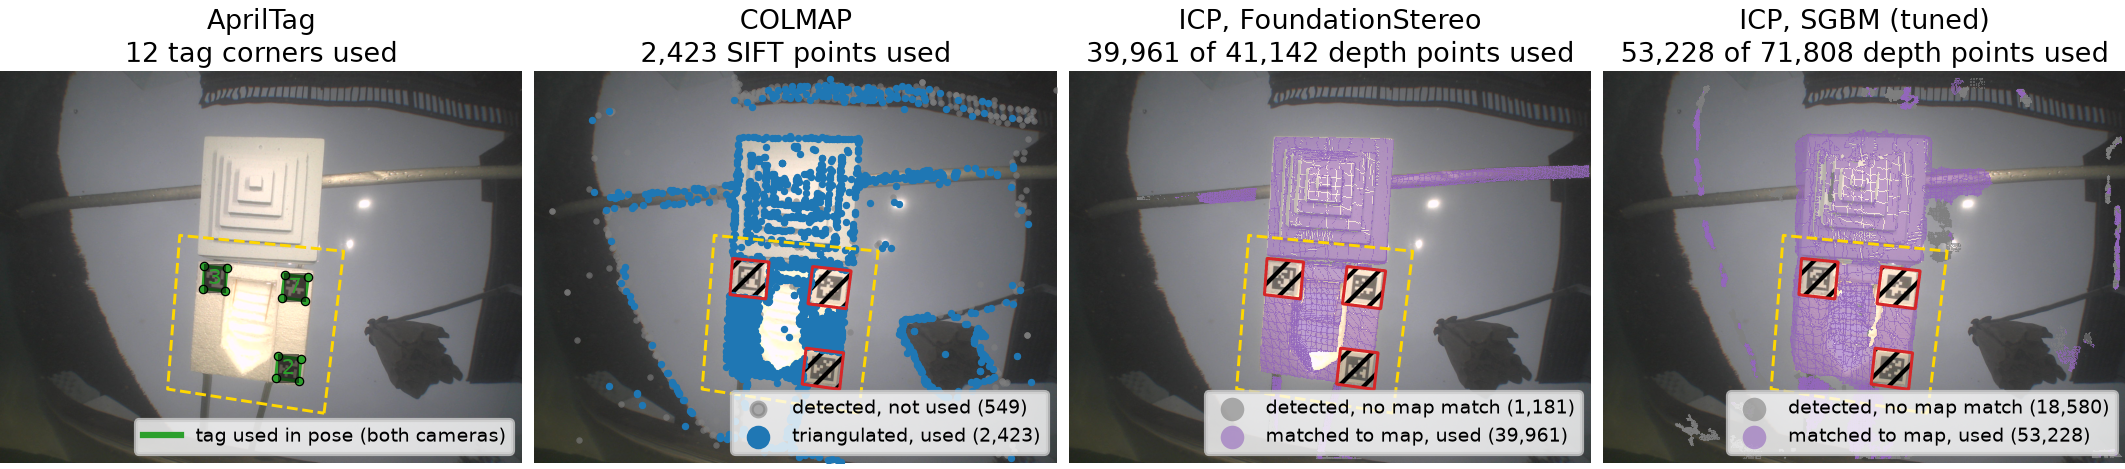
\includegraphics[width=1 \textwidth]{figs/Ch5/0060_all.png}
    \caption[Features used by each pose method]{Features used by each pose method in frame 60 of the shaded ice
    pass. The AprilTags are keep-out zones for the markerless methods, which cannot use any feature inside them.
    AprilTag: tags used in the pose. COLMAP: SIFT keypoints (blue: used; grey: unused). ICP: 2\,mm depth points
    (purple: matched within 5\,mm; grey: unmatched).}
    \label{fig:ch5.shadow_ice_detections}
\end{figure}



\subsection{Discussion}
\label{subsec:ch5.pose_discussion}
All three methods accurately estimate the camera pose relative to the target
in shaded conditions, but only ICP with FoundationStereo depth is able to
track the camera in sunlight. As shown in \autoref{fig:ch5.shadow_ice_detections}, all three methods also rely on
features outside the designed target. Although ICP with FoundationStereo is
the most consistent approach, further testing on an isolated ice target with
no background detail is needed to understand how the system will perform
beneath real ice.




%=====================================================================
% SECTION Fusing Frames
%=====================================================================
\section{Frame Fusion}
\label{sec:ch5.frame_integration}
% Intro to concept + Logic behind
Once each frame has both a depth map and a pose, they can be joined into a single model.
Each depth map is converted into a point cloud, and transformed into the world frame using its pose.

The points are combined with a technique called voxel voting. The space around the object is divided into small
cubes (voxels), and each frame votes for every voxel its points fall into. A voxel is only kept if sufficient frames
agree that the surface lies there. This rejects random points that only appear in a few frames. It also helps
to omit small floating particles that are not part of the scene, keeping only surfaces consistently seen from 
different viewpoints. 

The fused point cloud is then filtered to remove the remaining outliers, and, where relevant, aligned to the CAD model 
for scoring. 

\subsection{Fusion Methods}
\label{subsec:ch5.fusion_methods}
% Comparing different how our approach works


% Voxel voting (union) - keep every voxel that at least N frames hit - maybe a bit basicHO
% Median height field - for each x-y cell, take median height over the frames that it saw - assumes surface seen from one side, height over board, overhangs lost
% TSDF (truncated signed distance function) - each voxel stores a wighted average of a signed distance to a surfacce - THE STANDARD
% Point0cloud fusion (done by COLMAP) patchmap

% Explain the theory behind each type of fusing - use literature now while explaining , dont have to come bacek

% TSDF - standatd
%
\subsubsection{TSDF (Truncated Signed Distance Function)}
\label{subsec:ch5.tsdf}

The truncated signed distance function (TSDF) is the standard volumetric
representation for dense 3D reconstruction from depth data. Introduced by
Curless and Levoy~\cite{curlessVolumetricMethodBuilding1996}, it divides the scene
into a regular voxel grid. Each voxel $\mathbf{p}$ stores a signed distance
$F(\mathbf{p})$ to the nearest observed surface and a confidence weight
$W(\mathbf{p})$. Distances are positive in free space in front of the
surface and negative behind it, and are truncated to the interval
$[-\mu, \mu]$. Truncation keeps updates to a narrow band around the
surface. Each new depth frame $k$ produces a per-voxel
measurement $F_{R_k}(\mathbf{p})$ with weight $W_{R_k}(\mathbf{p})$. This
measurement is fused into the global model by a weighted running average:
\begin{equation}
  F_k(\mathbf{p}) =
  \frac{W_{k-1}(\mathbf{p})\,F_{k-1}(\mathbf{p}) + W_{R_k}(\mathbf{p})\,F_{R_k}(\mathbf{p})}
       {W_{k-1}(\mathbf{p}) + W_{R_k}(\mathbf{p})},
  \qquad
  W_k(\mathbf{p}) = \min\!\big(W_{k-1}(\mathbf{p}) + W_{R_k}(\mathbf{p}),\, W_{\max}\big).
  \label{eq:tsdf_fusion}
\end{equation}
Averaging over many frames suppresses sensor noise. The reconstructed
surface is recovered as the zero-level set $F(\mathbf{p}) = 0$, either by
raycasting or by extracting a mesh with Marching
Cubes~\cite{lorensen1987marching}. Because $F$ is continuous, interpolating
between voxels gives the surface at sub-voxel accuracy. 
In the implemented pipeline, the surface is extracted directly as a
point cloud using Open3D, placing a point wherever $F$ changes sign between neighbouring voxels.

\subsubsection{COLMAP Fusion}
\label{subsec:ch5.colmap_fusion}
% Take over to reconstruction section
Unlike the other two pose methods, COLMAP can also produce dense depth.
Once poses are known, it estimates depth for every pixel of each frame using PatchMatch multi-view stereo, 
comparing each pixel against multiple overlapping images rather than a single
stereo pair \cite{schonbergerPixelwiseViewSelection2016}. The depth maps are then fused into a single point cloud, 
keeping only points on which several depth maps agree.

% =======================================

\subsection{Test Setup}
\label{subsec:ch5.fusion_tested}

The depth map test (\autoref{sec:ch5.depth_test}) and pose test (\autoref{subsec:ch5.methods_tested}) produced a set of stereo depth maps and poses for each test dataset.
The COLMAP-generated poses are used for all of the fusion tests as COLMAP cannot take input poses.
This ensures all tests use the same poses. 
The test is run on S30 with 344 frame pairs (every fifth pair) with AprilTags masked out. Three different configurations are tested:

\begin{enumerate}
    \item \textbf{COLMAP pipeline:} COLMAP's PatchMatch stereo is run on the same structure-from-motion model
    that produced the poses. Each of the 688 images (left and right) gets its own depth map, matched against up
    to 20 neighbouring views, starting with its stereo partner. A $15\times15$\,px window is used at full
    resolution (1600\,px). COLMAP's stereo fusion then keeps a point only where at least 3 depth maps agree, with
    the tag masks applied at this step.
    \item \textbf{TSDF with SGBM depth maps:} one depth map per stereo pair (344), using the tuned SGBM settings
    from \autoref{sec:ch5.depth_test} at half scale.
    \item \textbf{TSDF with FoundationStereo depth maps:} one depth map per stereo pair (344), using the ViT-L
    model at half scale with the settings from \autoref{sec:ch5.depth_test}.
\end{enumerate}

Both TSDF runs use the same fusion settings: 1\,mm voxels, a truncation distance of 4\,mm, and a surface kept only
where at least 3 frames contributed. This is the TSDF equivalent of the voxel voting threshold. 

\subsection{Results}
\label{subsec:ch5.fusion_results}
The three fusion methods are first compared for accuracy and coverage on the 3D-printed targets, where the CAD
models provide ground truth. They are then compared based on reconstruction quality and coverage on the ice targets. Interactive
point clouds of all the reconstructions are available in the
\href{https://github.com/GlenOJones/UCT_Final_Year_Project}{\textcolor{blue}{GitHub repository}}.

% ====================
\subsubsection{Accuracy on 3D-Printed Targets (DS2)}
To measure accuracy, the 3D-printed objects are used (DS2), as their CAD models provide ground truth.
 The camera trajectory is aligned to the AprilTag poses so that every point cloud lies in the board frame. 
 Each object is cropped to a $\pm$85\,mm box around its known position, keeping only the points above the board 
 that belong to the object. The CAD model is fitted to these points by point-to-plane ICP. 
     Accuracy is then measured as the signed distance
    from each point to the CAD surface. The median absolute distance is the main comparison metric, because it is robust to outliers.
     Coverage is the percentage of the visible CAD surface that has a reconstructed point within 2\,mm. 
     It shows how much of the shape was captured.
     Only one of the two egg carton tiles (\autoref{fig:ch5.printed_shapes}) is included. The other was not
     reconstructed well enough by any of the three methods for the CAD model to be fitted reliably by ICP, so it
     could not be scored.

\begin{table}[H]
\centering
\small
\setlength{\tabcolsep}{5pt}
\caption{Accuracy of each fusion method against the CAD models on S30 (344 frames, COLMAP poses, tags
masked). Best value per object in bold.}
\label{tab:fusion_accuracy}
\begin{tabular}{llrrr}
\toprule
Object & Method & Cov. (\%) & Median $|d|$ (mm) & RMS (mm) \\
\midrule
\multirow{3}{*}{Pyramid}         & COLMAP    & 36          & 3.23          & 3.91          \\
                                 & TSDF-FS   & \textbf{40} & 2.21          & \textbf{2.53} \\
                                 & TSDF-SGBM & 17          & \textbf{2.05} & 3.35          \\
\midrule
\multirow{3}{*}{Pyr. 2$\times$2} & COLMAP    & 43          & 1.93          & 2.59          \\
                                 & TSDF-FS   & \textbf{44} & \textbf{1.72} & \textbf{2.27} \\
                                 & TSDF-SGBM & 35          & 2.51          & 5.03          \\
\midrule
\multirow{3}{*}{Egg carton}      & COLMAP    & 35          & \textbf{1.83} & \textbf{2.90} \\
                                 & TSDF-FS   & 21          & 3.83          & 5.81          \\
                                 & TSDF-SGBM & \textbf{36} & 2.37          & 5.02          \\
\bottomrule
\end{tabular}
\end{table}


\begin{figure}[H]
    \centering
    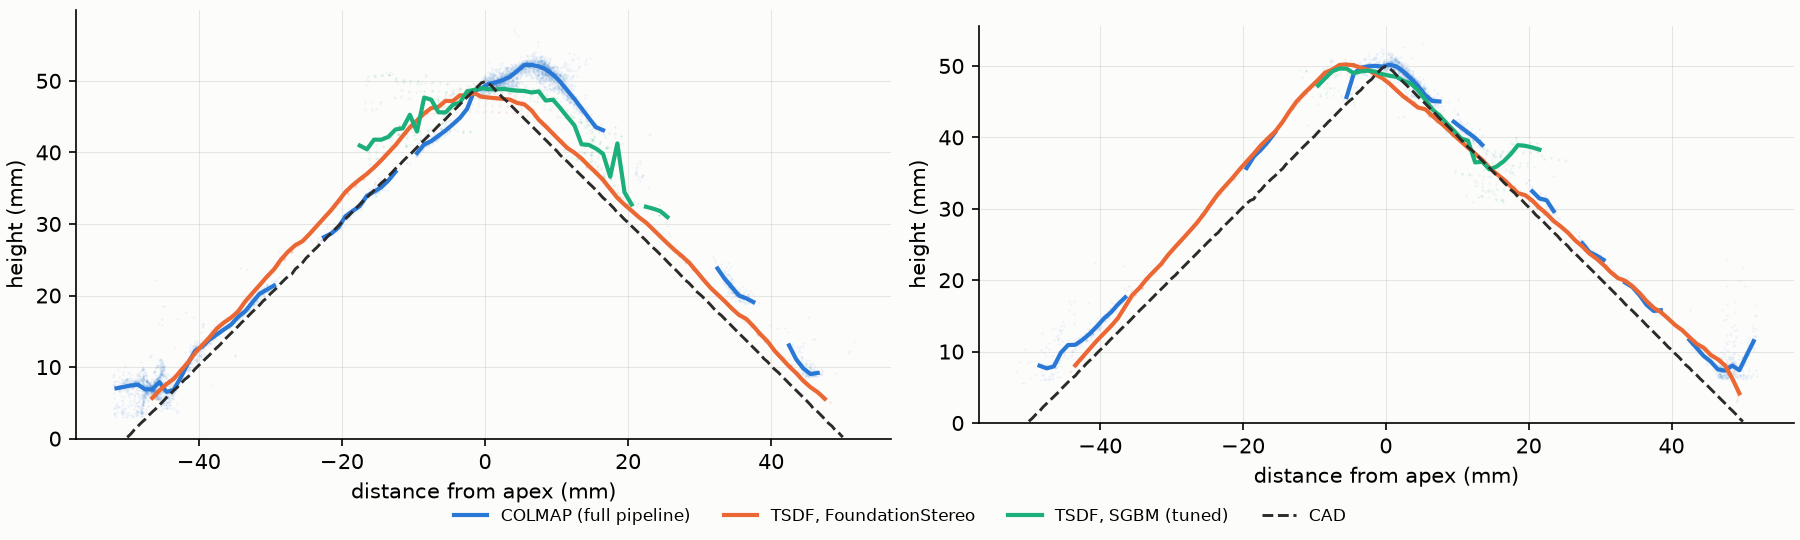
\includegraphics[width=\textwidth]{figs/Ch5/fusion_profiles_pyramid.png}
    \caption[Profiles through the pyramid apex]{\textbf{Profiles through the pyramid apex.} Each fusion method
    against the CAD model (dashed), along its $x$ axis (left) and $y$ axis (right). Lines show the median height of
    the scan points near the section, with the points shown faintly. Only TSDF with FoundationStereo gives a
    continuous profile. All three methods sit 2--4\,mm above the CAD surface.}
    \label{fig:ch5.fusion_profiles_pyramid}
\end{figure}

\begin{figure}[H]
    \centering
    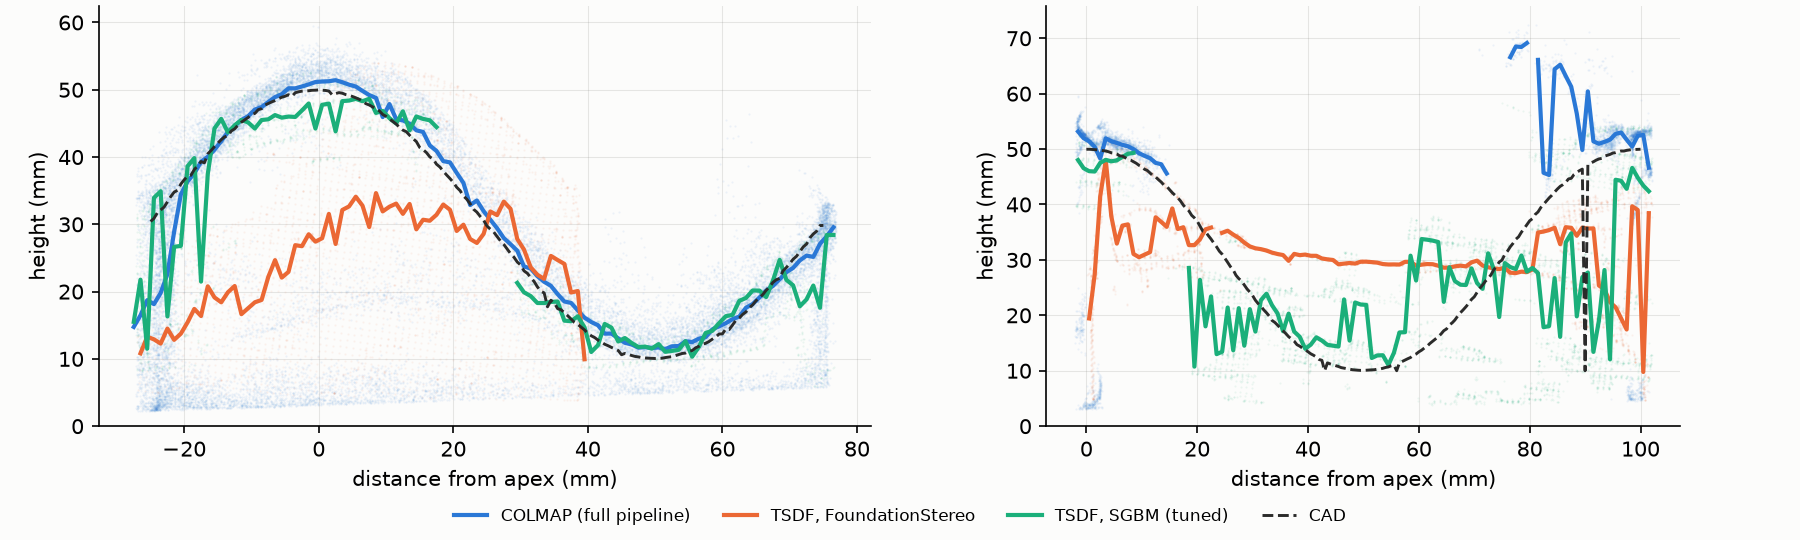
\includegraphics[width=\textwidth]{figs/Ch5/fusion_profiles_egg.png}
    \caption[Profiles through the egg carton apex]{\textbf{Profiles through the egg carton apex.} Each fusion method
    against the CAD model (dashed), along its $x$ axis (left) and $y$ axis (right), drawn as in
    \autoref{fig:ch5.fusion_profiles_pyramid}. Along $x$, COLMAP and SGBM follow the designed curve, while TSDF
    with FoundationStereo sits 15--20\,mm low over the bump. Along $y$, all three methods are noisy.}
    \label{fig:ch5.fusion_profiles_egg}
\end{figure}

TSDF with FoundationStereo performed best on the pyramids, with the highest coverage and the lowest RMS error on
both. Its only weaker result was the median error on the single pyramid, which was slightly higher than that of
TSDF with SGBM (2.21 against 2.05\,mm). The profiles in \autoref{fig:ch5.fusion_profiles_pyramid} support this.
TSDF with FoundationStereo is the only method that follows the entire surface. It does, however,  consistently sit a few
millimetres above the CAD surface. This may account for its slightly
higher median error.

The egg carton tells a different story, with TSDF with FoundationStereo clearly the worst of the three methods.
In \autoref{fig:ch5.fusion_profiles_egg}, COLMAP tracks the designed curve almost perfectly along the $x$ axis,
but falls apart along the $y$ axis, where it has no points inside the dip. COLMAP also places
points inside the solid part of the object, visible below the curve in the $x$ profile as the faint dots. TSDF with SGBM sits
between the other two. Its profiles are fairly complete, giving it the highest coverage (36\,\%), but they are
noisy, which raises its RMS error. TSDF with FoundationStereo flattens the dip, placing a surface where there is
none. This drives up its error, with the highest median and RMS of any method, and it also has the lowest
coverage (21\,\%).

%=======================================================
\subsubsection{Reconstructions of Ice Targets (DS3)}

% Explain what was done

% Explain that its largely qualittave comparison, no ground truth. I would like to compare %coverage tho
The ice targets have no CAD model, meaning their reconstructions cannot be scored for accuracy. The comparison is
therefore largely qualitative, based on how clean and complete the reconstructions look. 
 \autoref{fig:ch5.fusion_oblique} shows each method's reconstruction of the four targets in shaded conditions.

\begin{figure}[H]
    \centering
    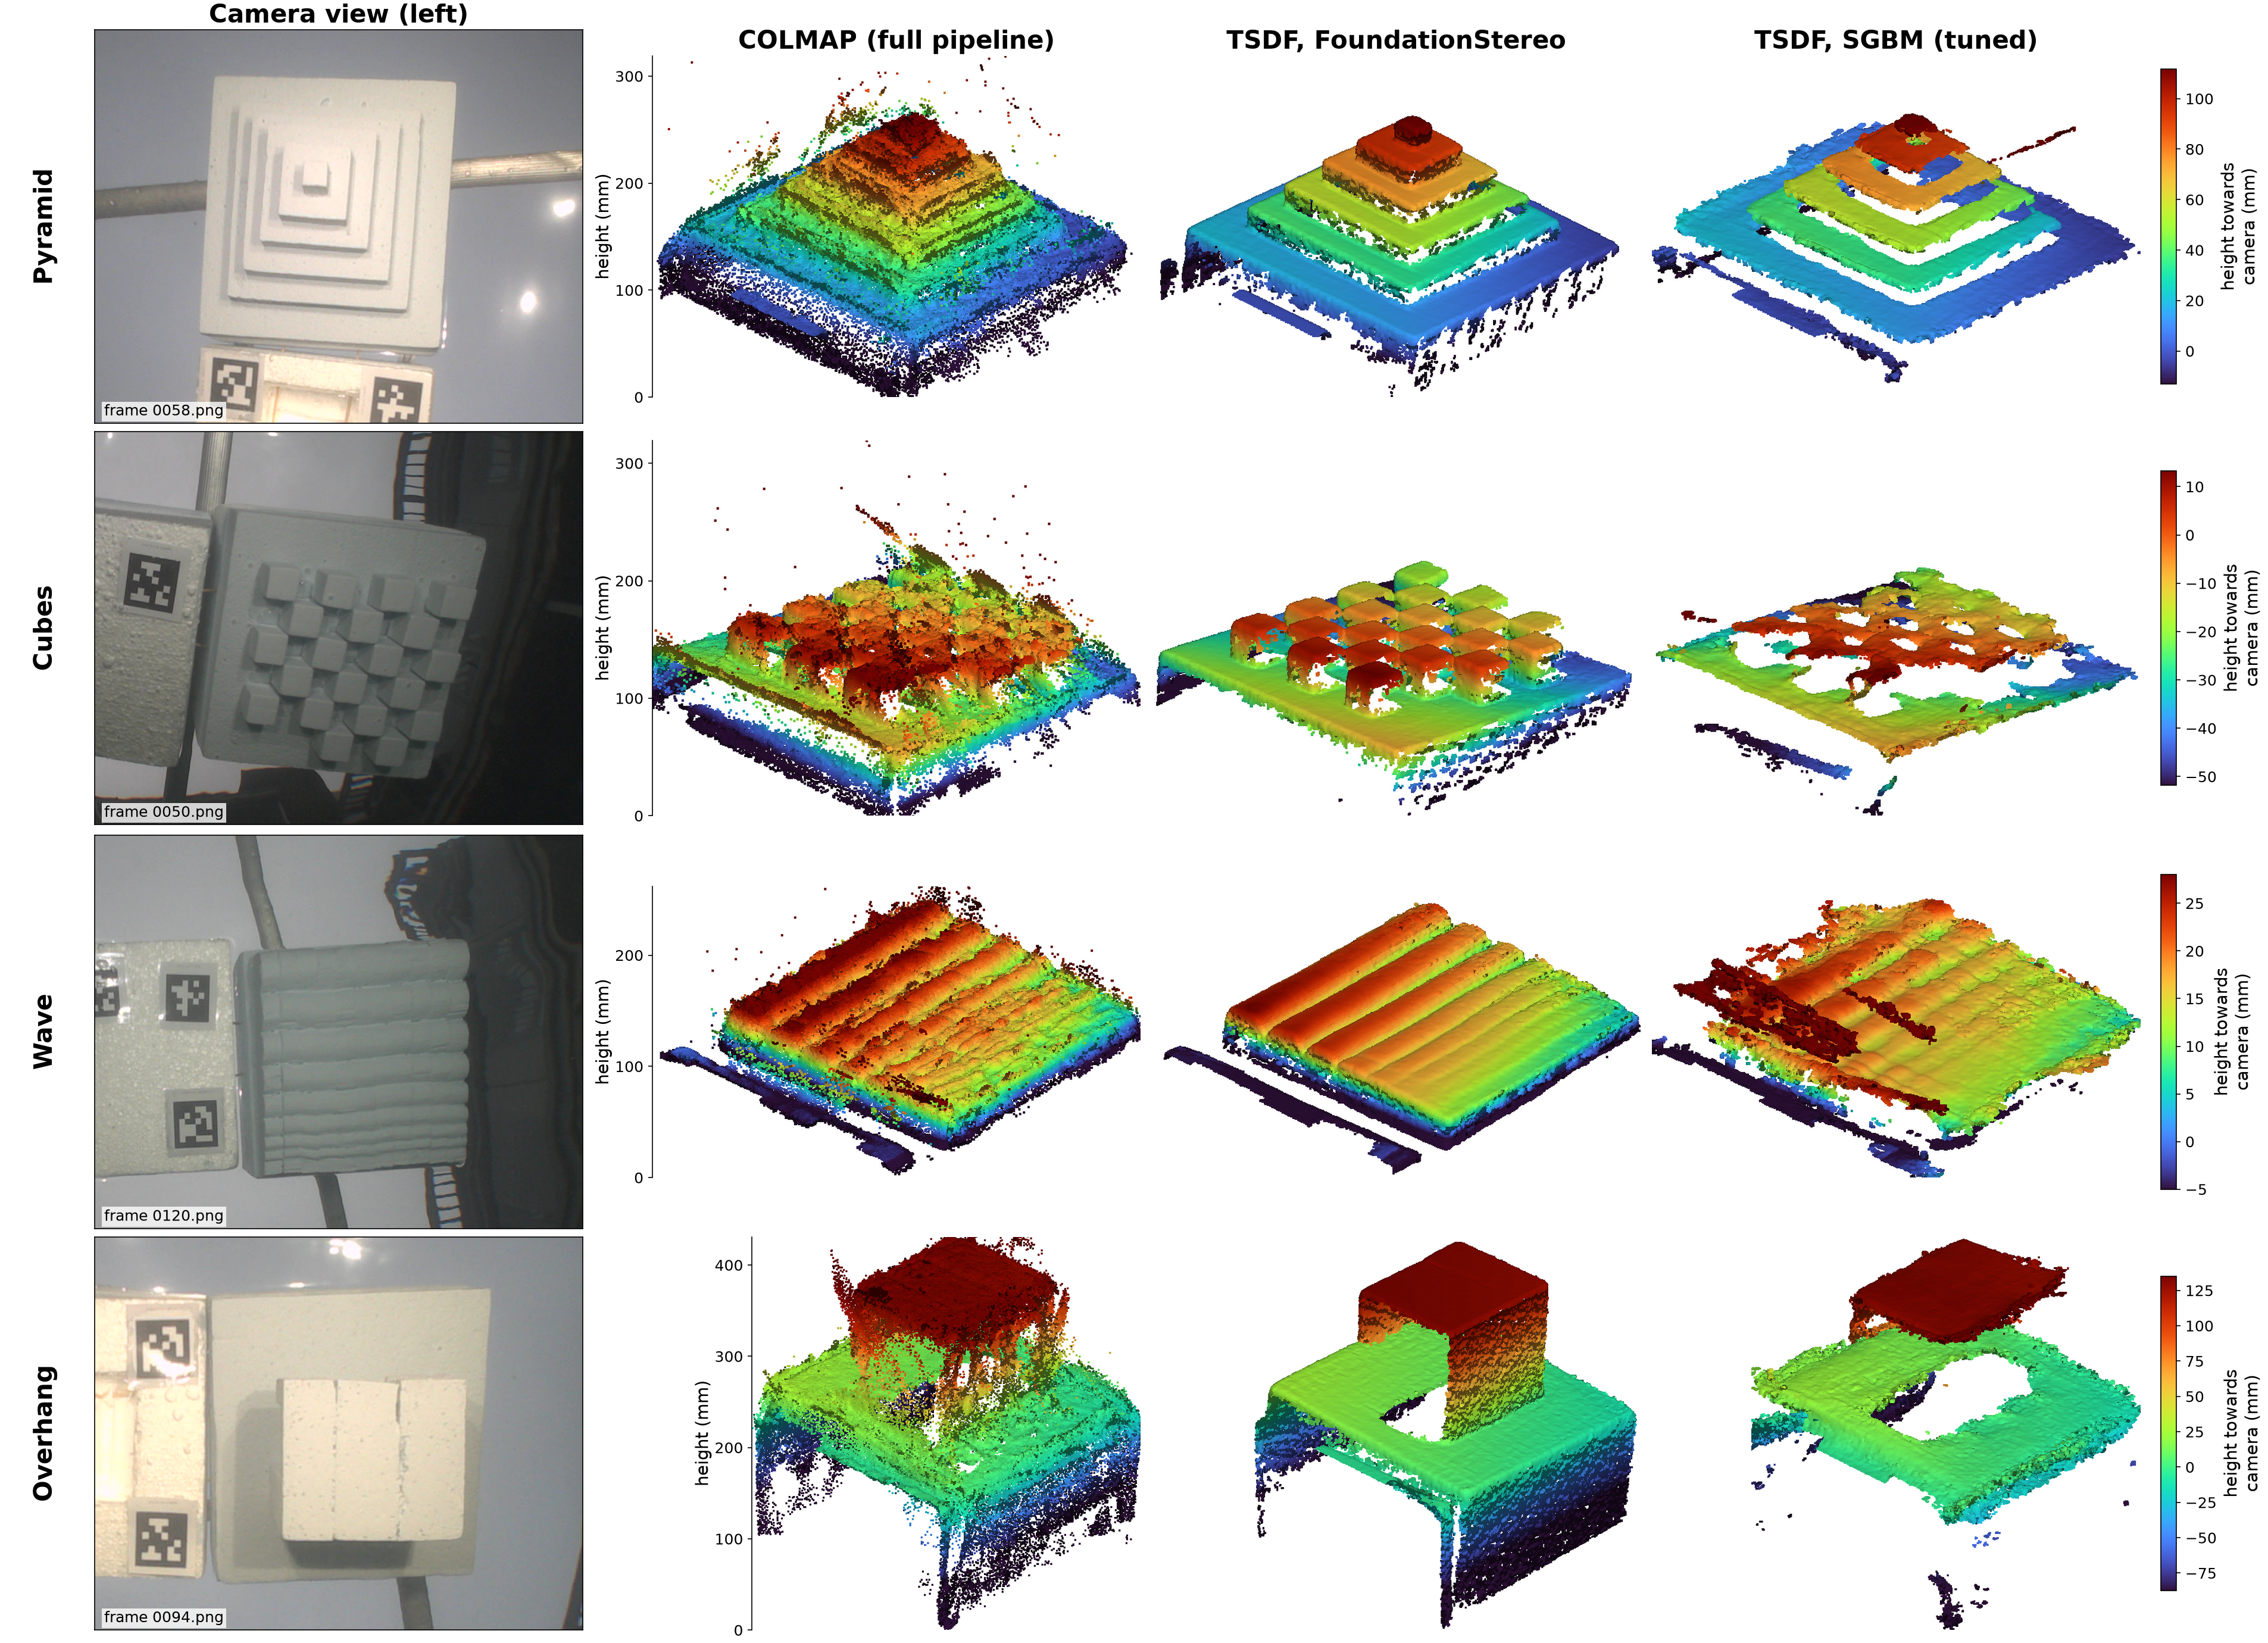
\includegraphics[width=\textwidth]{figs/Ch5/fusion_oblique_grid_with_image.png}
    \caption[Oblique views of the fused ice reconstructions]{\textbf{Oblique views of the fused ice
    reconstructions.} Left: a camera frame of each ice target. Right: each fusion method's point cloud, viewed
    from 30$^\circ$ above the board and coloured by height above the board. Each row has its own colour scale
    and is scaled to fill the row, so the rows cannot be compared by size. The ruler shows true lengths for
    vertical features only; heights above the board are given by the colour scale.}
    \label{fig:ch5.fusion_oblique}
\end{figure}

% Add github link with cloud viewer

All three methods recover the overall shape of each ice target, but \autoref{fig:ch5.fusion_oblique} 
shows clear differences in how cleanly they do so. COLMAP produces the most noise, with points generated where there are no surfaces. 
Scattered points float above every COLMAP-generated target, and 
on the overhang, streaks of points hang down from the edges of the top block.
 Its surfaces are also rougher, with the pyramid steps and the cubes blurred by noise.

  TSDF with SGBM depth maps gives a cleaner but less complete reconstruction. It captures surfaces facing the camera, 
  such as the tops of the pyramid steps and the overhang, but loses the steep faces between them. This
  leaves holes in the base and gaps between the steps. It also merges the cubes into a single patch at
  the back right corner. 
  
   TSDF with FoundationStereo gives the cleanest visual result on every target.
   The pyramid steps are sharp and flat and each cube is separated from its neighbours. All of the waves are visible, 
   and the overhang is recovered along with its side walls. 


\subsection{Discussion}
\label{subsec:ch5.fusion_discussion}
% FS Best allrounder
No fusion method performed best on every object when both accuracy and reconstruction quality are considered.
TSDF with FoundationStereo depth maps gave the most complete and most accurate reconstructions of both pyramids,
as well as the cleanest results on all four ice targets. However, it was the least accurate on the egg carton.

TSDF with SGBM had the lowest median error on the single pyramid, but only because it reconstructed the easiest
17\,\% of the surface, around the apex. On the 2$\times$2 pyramid and the egg carton its RMS error is about twice
its median, meaning a few points lie far from the surface, matching the speckle in its depth maps
(\autoref{sec:ch5.depth_test}). For TSDF with FoundationStereo and COLMAP on the pyramids, the RMS error is only
1.1--1.3 times the median, implying a near-constant offset rather than noise. This matches the 2--4\,mm offset
in \autoref{fig:ch5.fusion_profiles_pyramid}. 

The egg carton is smooth, has very little texture, and the inside of each curve is partly hidden from the camera.
The likely cause is that, where FoundationStereo cannot find reliable matches, the learnt model fills the gap with
a smooth, near-flat surface rather than the true curve. COLMAP and SGBM also struggle inside the dip, but they leave
gaps or noise there, whereas FoundationStereo produces a plausible surface that is wrong, which is harder to detect.
For the ice targets (DS3), TSDF with FoundationStereo gave noticeably cleaner reconstructions across all four tests.

TSDF with FoundationStereo is therefore chosen as the default fusion method, with the caveat that it may smooth
out curved areas that are partly hidden from the camera. All three methods remain available in the pipeline. For
real ice deployments, it is recommended to run both COLMAP and TSDF with FoundationStereo on the same data, and to
compare the two to find where FoundationStereo may have filled in surface that is not there.


% /home/remote/Desktop/GlenRemote/UCT_Final_Year_Project/data/3DRecon/3DPrintFinal/30_frames_range (S30)

% /home/remote/Desktop/GlenRemote/UCT_Final_Year_Project/data/3DRecon/Ice/Cubes/Shade/cub2_frames_horiz_pass_v_close_580mm/ (CUBES)
% /home/remote/Desktop/GlenRemote/UCT_Final_Year_Project/data/3DRecon/Ice/Overhang/Shade/hang1_frames_pass2_830mm/ (Overhang Shade)
% /home/remote/Desktop/GlenRemote/UCT_Final_Year_Project/data/3DRecon/Ice/Wave/Shade/wave1_frames_pass2_720mm/ (wave)

%=====================================================================
% SECTION: Full Pipeline Performance
%=====================================================================


\section{Importance of Frame Count Across the Whole Pipeline}
\label{sec:ch5.testing_full_pipeline}

During a real under-ice pass the ROV moves faster than in the recorded scans, so each surface is seen in fewer, more widely
spaced frames. Motion blur cannot be reproduced from the existing recordings, but the effect of fewer frames can.
The four shaded ice targets from DS3 are therefore re-run through the full pipeline using only every
$N$\textsuperscript{th} frame, for $N = 1, 2, 8,$ and $16$. The
effect on the poses and reconstructions is measured, along with the time of each stage.


\subsection{Coverage Against Frame Count}

\begin{figure}[H]
    \centering
    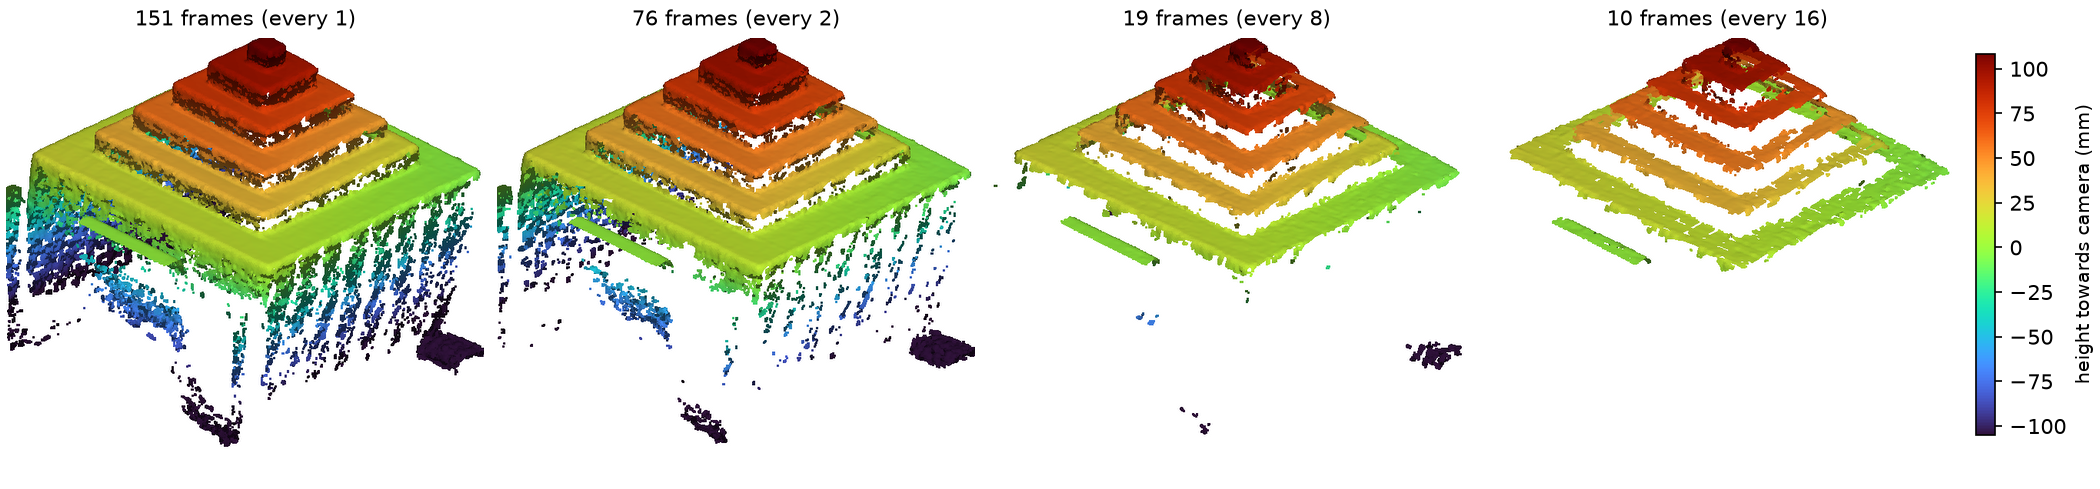
\includegraphics[width=\textwidth]{figs/Ch5/frame_count_oblique_by_frames.png}
    \caption[Pyramid ice reconstructions against frame count]{\textbf{Pyramid ice reconstructions against frame
    count.} TSDF reconstructions of the shaded pyramid with FoundationStereo depth, using every 1st, 2nd, 8th and
    16th frame (151 frames down to 10), shown from the same oblique view. Points are coloured by height towards the
    camera.}
    \label{fig:ch5.frame_count_oblique_pyramid}
\end{figure}

\begin{figure}[H]
    \centering
    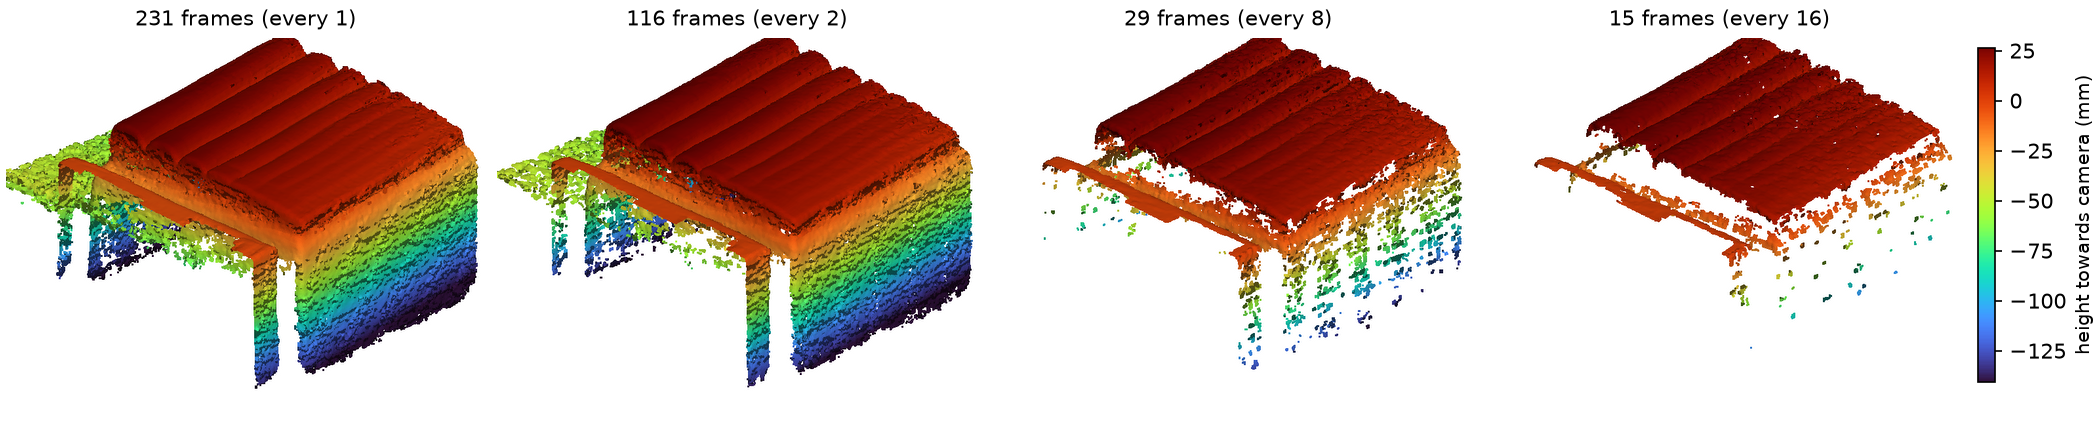
\includegraphics[width=\textwidth]{figs/Ch5/frame_count_oblique_by_frames_wave.png}
    \caption[Wave ice reconstructions against frame count]{\textbf{Wave ice reconstructions against frame
    count.} TSDF reconstructions of the shaded wave with FoundationStereo depth, using every 1st, 2nd, 8th and
    16th frame (231 frames down to 15), shown from the same oblique view. Points are coloured by height towards the
    camera.}
    \label{fig:ch5.frame_count_oblique_wave}
\end{figure}

As the number of frames is reduced, the surfaces facing the camera remain well reconstructed, while the side walls lose
their coverage (\autoref{fig:ch5.frame_count_oblique_pyramid} and \autoref{fig:ch5.frame_count_oblique_wave}). This is
expected, as the side walls are only visible in a few frames near the edges of the pass, whereas the faces towards the
camera are seen in almost every frame. As a result, the pyramid and cubes break up more quickly. The steps of the
pyramid and the sides of the cubes are quickly lost, leaving gaps between the faces that remain. The smoother wave
surface stays mostly complete, even with only 15 frames. The reconstructions of all four targets are given in the appendix
(\autoref{fig:app.frame_count_oblique_all}).

\subsection{Timing and Compute Usage}

\autoref{tab:frame_count_full_runs} gives the time of each stage for the full runs on each target. Total run time
was mainly influenced by the number of frames. The targets took 6.7--7.7\,s per frame. FoundationStereo runs a fixed number of iterations, 
so its time per frame was
nearly constant, and TSDF fusion was negligible. Only COLMAP varied with the target, as its iterative matching and
bundle adjustment grow with the number of keypoints. The cubes, with the most corners and edges, were the slowest
per frame.

\begin{table}[H]
\centering
\small
\caption{Time of the full runs (every frame) of the final pipeline on each ice target: each stage's time per
frame in seconds, and the total time of the run in minutes. Per-frame times are from the stage times in minutes, so
the stages may not sum exactly to the total.}
\label{tab:frame_count_full_runs}
\begin{tabular}{lrrrrrr}
\toprule
 & \multicolumn{4}{c}{Time per frame (s)} & & \\
\cmidrule(lr){2-5}
 & Poses & Depth & Fusion & & & Total \\
Target & (COLMAP SfM) & (FoundationStereo) & (TSDF) & Total & Frames & (min) \\
\midrule
Pyramid  & 2.54 & 4.33 & 0.12 & \textbf{6.99} & 151 & 17.6 \\
Cubes    & 3.30 & 4.40 & 0.09 & \textbf{7.74} & 131 & 16.9 \\
Wave     & 2.60 & 4.42 & 0.16 & \textbf{7.17} & 231 & 27.6 \\
Overhang & 2.27 & 4.27 & 0.14 & \textbf{6.68} & 211 & 23.5 \\
\bottomrule
\end{tabular}
\end{table}

\subsection{Discussion}
Even a pass with a few frames still reconstructs the surfaces facing the camera. Steep features, such as the sides of ridges and blocks, need more frames, so a
slower pass or several passes would be needed to capture them. 

The processing time is dominated by FoundationStereo: a pass of about 200 frames takes roughly 25 minutes to process, which is practical for
post-processing but not for real-time use.



%=====================================================================
% SECTION: Chapter Summary
%=====================================================================
\section{Reconstruction Conclusion}
\label{sec:ch5.summary}
This chapter built and tested the reconstruction pipeline one stage at a time. For depth, FoundationStereo gave
the most complete depth maps on the ice in shade and was the only matcher to keep the full ice shape when backlit
by the sun. For pose, COLMAP was the most accurate method in shade, with an ATE of 6.8\,mm on the pyramid ice
against 25--30\,mm for ICP, although only ICP with FoundationStereo depth kept tracking in direct sunlight. For
fusion, TSDF with FoundationStereo depth gave the most complete and accurate reconstructions of both pyramids and
the cleanest results on the ice targets, with median errors of around 2\,mm against the CAD models. Reducing the
number of frames mainly removed the side walls, while the surfaces facing the camera were kept even with
10--15 frames.

The final default pipeline is therefore COLMAP for pose, FoundationStereo for depth and TSDF for fusion, taking
around 7\,s per frame. Three limitations of the pipeline were flagged. FoundationStereo can flatten smooth, low-texture curves, as on the
egg carton. Direct sunlight reduces the depth coverage of every matcher, and all of the markerless pose methods
relied partly on features outside the targets. These are further discussed in \autoref{ch:discussion}.